%! Author = bedlamzd
%! Date = 16.02.2021

% Preamble
\documentclass[14pt]{extarticle}

%! Author = bedlamzd
%! Date = 16.02.2021

\usepackage{fontspec}
\usepackage{polyglossia}
\defaultfontfeatures{Ligatures=TeX}
\setdefaultlanguage{russian}
\setotherlanguage{english}
\setmainfont{PT Astra Serif}
\newfontfamily{\latinfont}{PT Astra Serif}
\newfontfamily{\cyrillicfont}{PT Astra Serif}
\newfontfamily{\cyrillicfonttt}{FreeMono}

\usepackage{geometry}

\usepackage{amsmath}
\usepackage{amssymb}
\usepackage{amsfonts}
\usepackage{graphicx}
\usepackage{float}
\usepackage{wrapfig}
\usepackage[caption=false]{subfig}

\geometry{right=20mm}
\geometry{left=20mm}
\geometry{top=20mm}
\geometry{bottom=20mm}

\usepackage{indentfirst}
\usepackage[outputdir=out]{minted}

\renewcommand{\theFancyVerbLine}{\ttfamily{\normalsize\oldstylenums{\arabic{FancyVerbLine}}}}

\newminted{python}{autogobble, linenos, fontsize=\small, xleftmargin=2\parindent}
\newmintinline{python}{fontsize=\small}
\newmintedfile{python}{autogobble, linenos, fontsize=\small, xleftmargin=2\parindent,
breakanywhere, breaklines}

\renewcommand{\thesubsection}{\arabic{subsection}}

\graphicspath{{../img/}}



% Document
\begin{document}
    \begin{center}
        \Large Лабораторная работа 1. Введение в анализ данных с Python
    \end{center}
    \begin{flushleft}
        \textbf{Имя:} Борисов Максим

        \vspace{1em}
        \textbf{Номер в ИСУ:} 225169

        \vspace{1em}
        \textbf{Группа:} R41341C
    \end{flushleft}

    \section*{Задание}
    Есть набор данных, который содержит данные о напряжении, токе и времени измерения. Период измерения 0,001 с.
    Период тестового сигнала 0,1 с. Количество периодов тестового сигнала - 1000. Тип двигателя - двигатель
    постоянного тока.

    \vspace{1em}
    Необходимо
    \begin{enumerate}
        \item Импортировать библиотеки
        \item Загрузить и подготовить данные
        \item Отобразить графики тока и напряжения
        \item Рассчитать значения параметров L и R
        \item Рассчитать средние значения и стандартное отклонение параметров L и R
    \end{enumerate}

    \pagebreak

    \subsection{Импортирование библиотек}
    \pythonfile[firstline=1, lastline=4]{../src/main.py}
    Библиотека \pythoninline/typing/ необходима для указания сигнатур функций для удобства работы в IDE.

    \subsection{Загрузка и подготовка данных}
    \pythonfile[firstline=17, lastline=25]{../src/main.py}

    Значение напряжения и времени 11-го элемента массива: t = 0.011; U = 1

    \subsection{Графики тока и напряжения}
    \pythonfile[firstline=42, lastline=60]{../src/main.py}

    \begin{figure}[H]
        \centering
        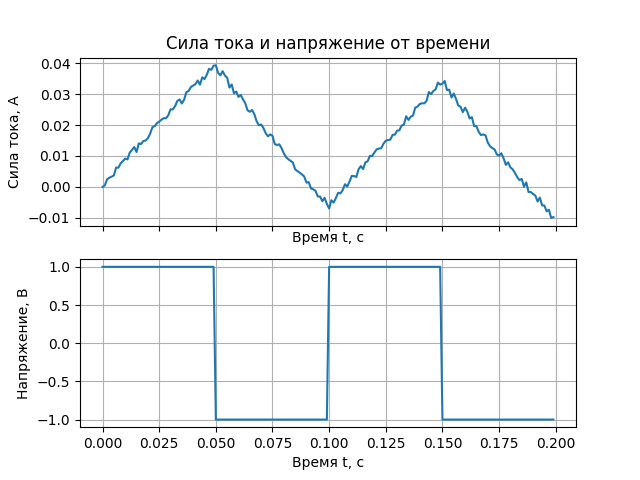
\includegraphics[width=\linewidth]{current-voltage-2T.png}
        \caption{График тока и напряжения от времени}
    \end{figure}

    \subsection{Рассчёт параметров L и R}
    Функция расчёта параметров L и R. Проверки коэффициентов k (например на равенство нулю) не требуется,
    так как для numpy это вызовет лишь warning, а не exception и значения в дальнейшем легко отфильтровать.
    \pythonfile[firstline=7, lastline=13]{../src/main.py}

    Расчёт параметров на всей выборке и отображение графиков.
    \pythonfile[firstline=62, lastline=80]{../src/main.py}

    \begin{figure}[H]
        \centering
        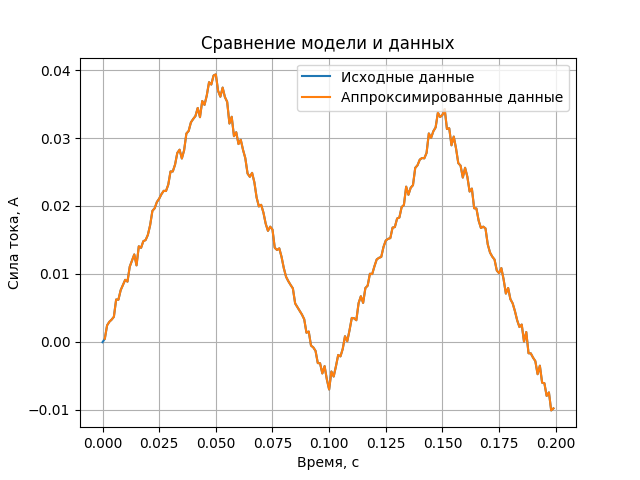
\includegraphics[height=0.4\textheight]{current_estimation_comparison.png}
        \caption{Сравнение реальных данных и модели}
    \end{figure}

    Значения параметров: $R = 8\ \text{Ом}$, $L = 1.17\ \text{Гн} $

    \subsection{Рассчёт среднего значения и стандартного отклонения параметров L и R}
    \pythonfile[firstline=82]{../src/main.py}

    \begin{table}[H]
        \centering
        \begin{tabular}{|c|c|c|}
            \hline
            & R, Ом & L, Гн \\ \hline
            Медиана & 8.04  & 1.17  \\ \hline
            СКО     & 1.82  & 0.02  \\ \hline
        \end{tabular}
    \end{table}

    \pagebreak
    \section*{Полный код}
    \pythonfile{../src/main.py}

\end{document}
